\chapter{Systems diagrams}
\label{ap:Algorithms}
\graphicspath{{Appendix4/Appendix4figures/}}

\section{Interface}

The software's main interface and clashlist is show in Figure \ref{fig:fig:mainInterface} and Figure \ref{fig:fig:clashInterface}.

\begin{figure}
  \centering
  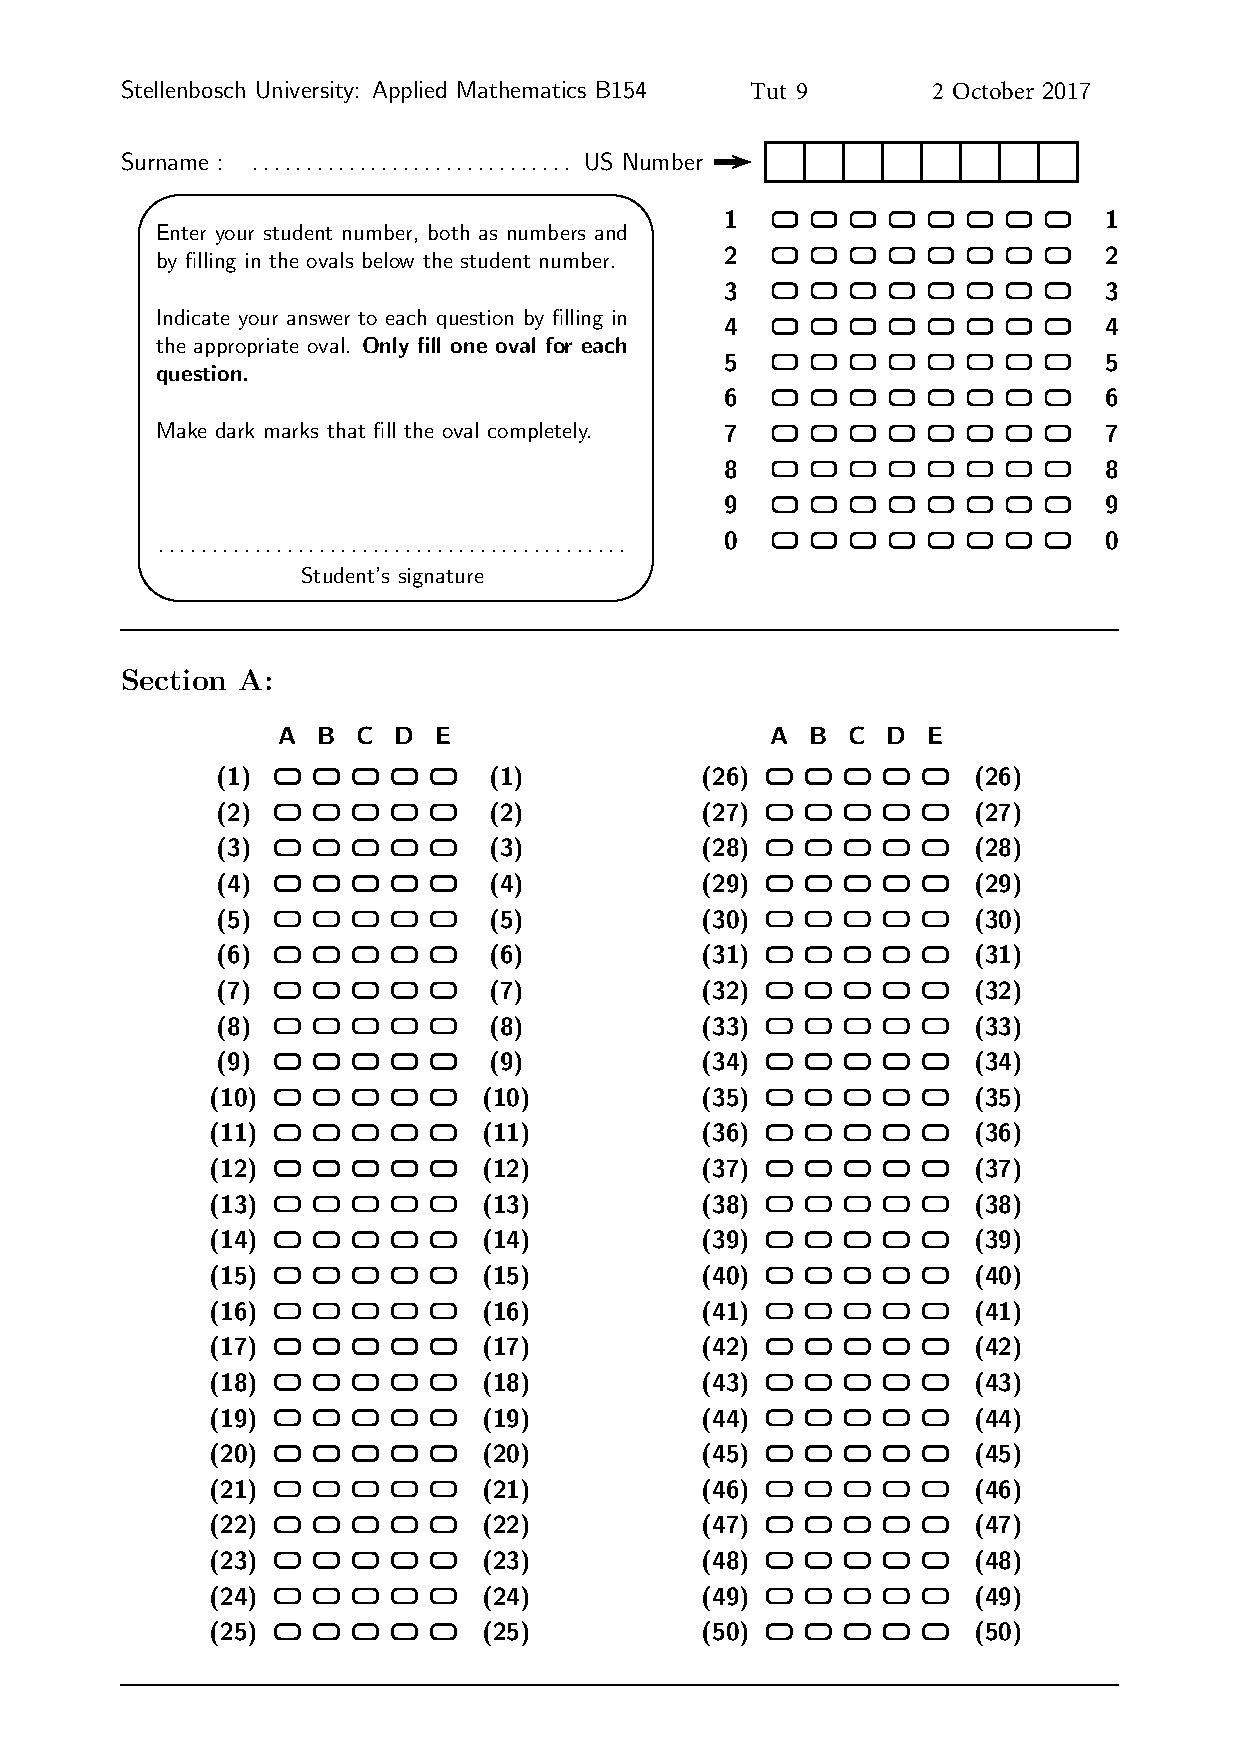
\includegraphics[width=8cm]{mainInterface}\\
  \caption{Main interface of test grader.}
  \label{fig:mainInterface}
\end{figure}

\begin{figure}
  \centering
  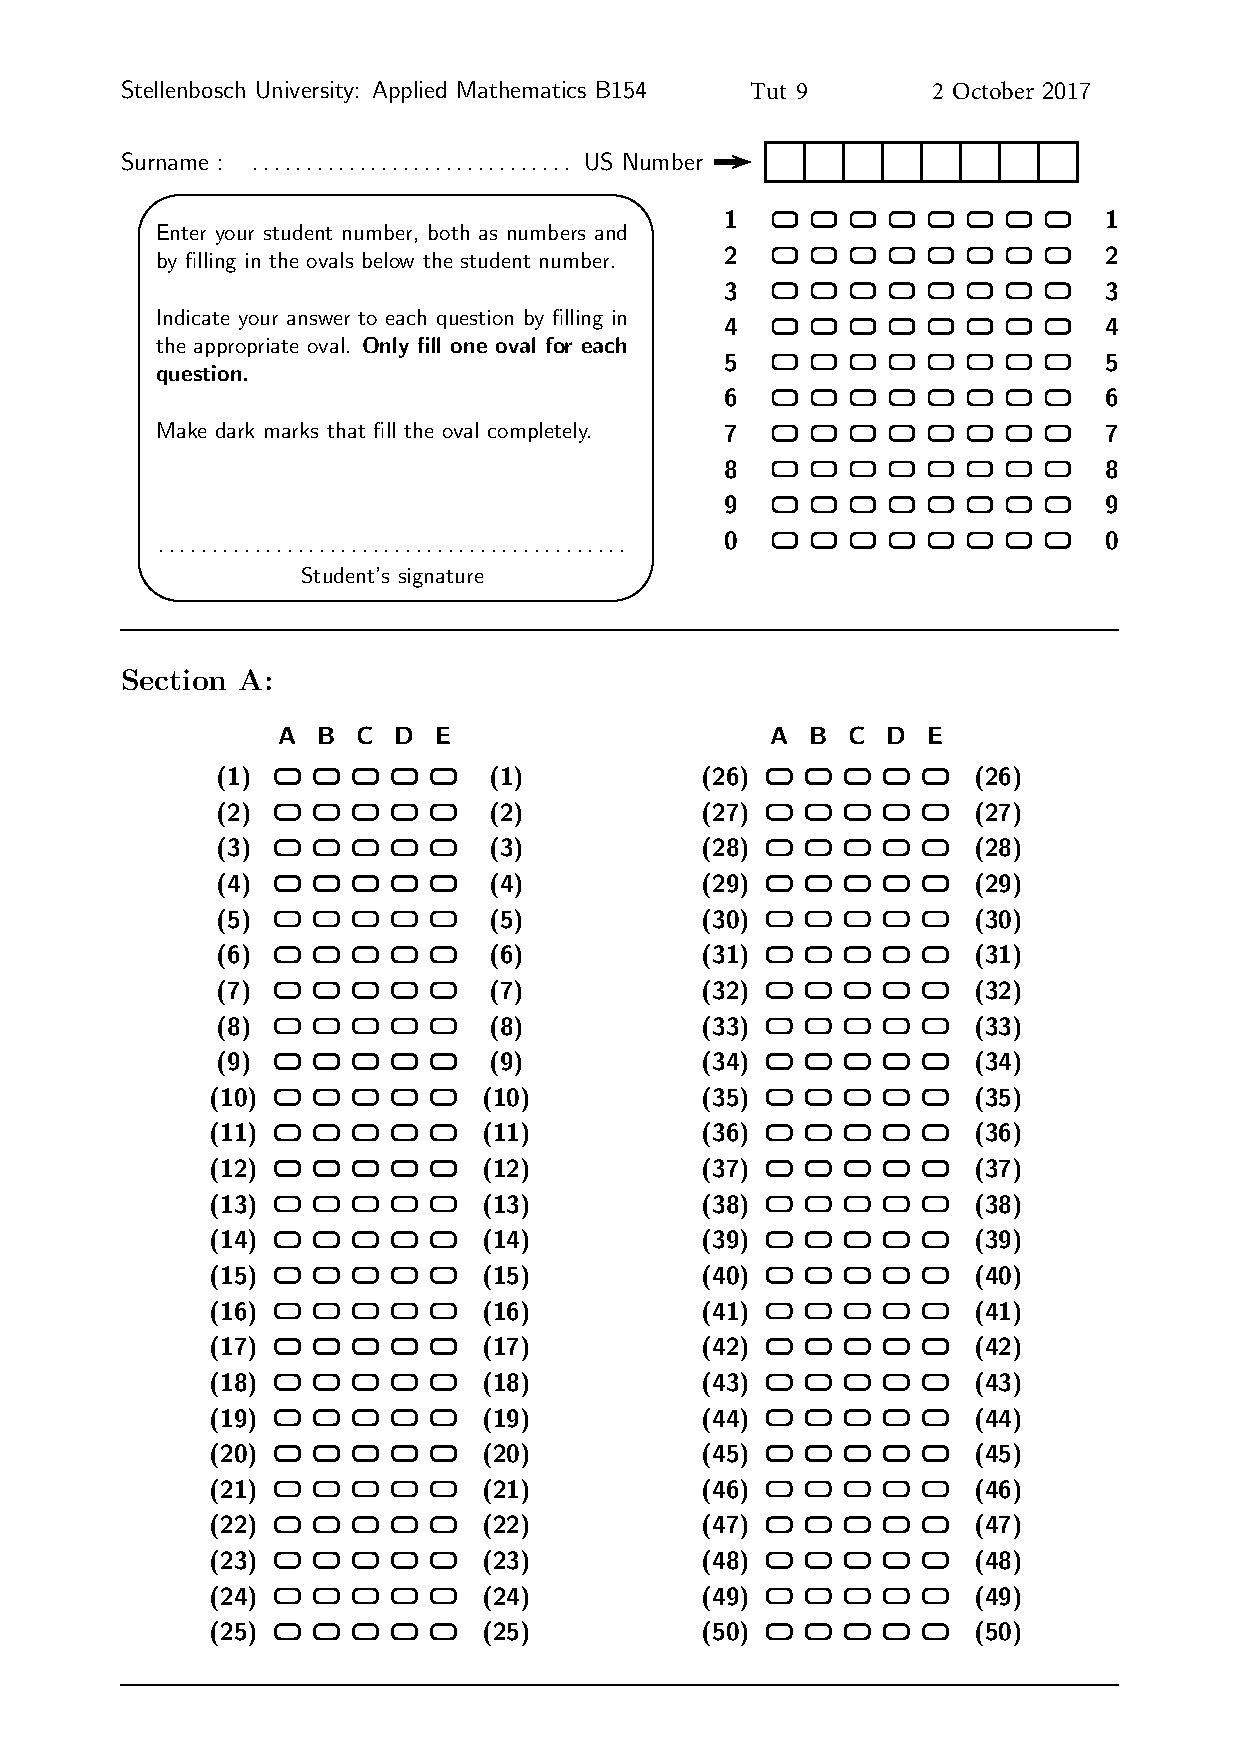
\includegraphics[width=8cm]{clashInterface}\\
  \caption{Clashlist interface of test grader.}
  \label{fig:clashInterface}
\end{figure}

\section{Templates}

The original template can be seen in the Figures \ref{fig:fig:template1}. 

\begin{figure}
  \centering
  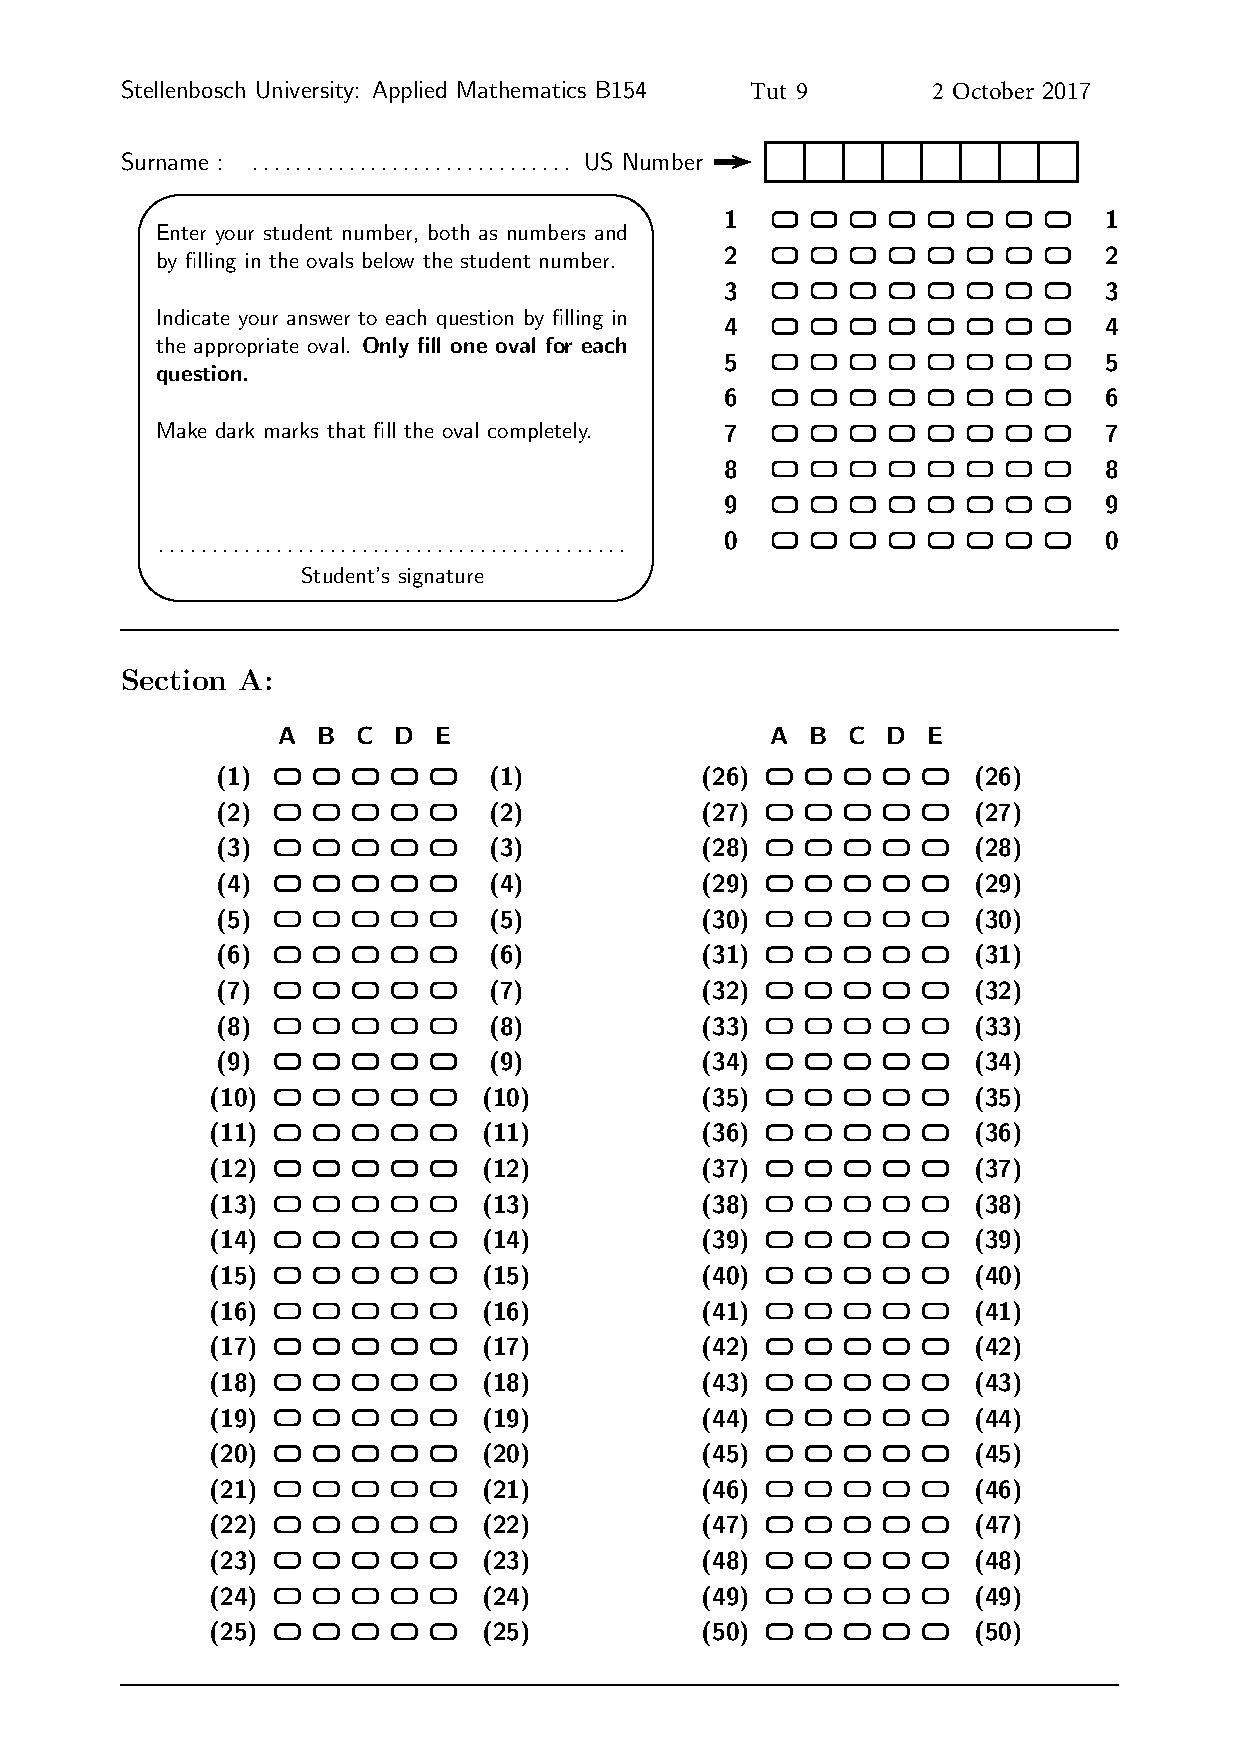
\includegraphics[width=8cm]{template1}\\
  \caption{Original template focussed on numbered answered questions.}
  \label{fig:template1}
\end{figure}

Two additional templates has also been developed and implemented for the department. These templates gives the department the capabilities of grading numbered answered questions as well as multiple choice questions. These templates are shown in Figure \ref{fig:fig:template2} and Figure \ref{fig:fig:template3}.

\begin{figure}
  \centering
  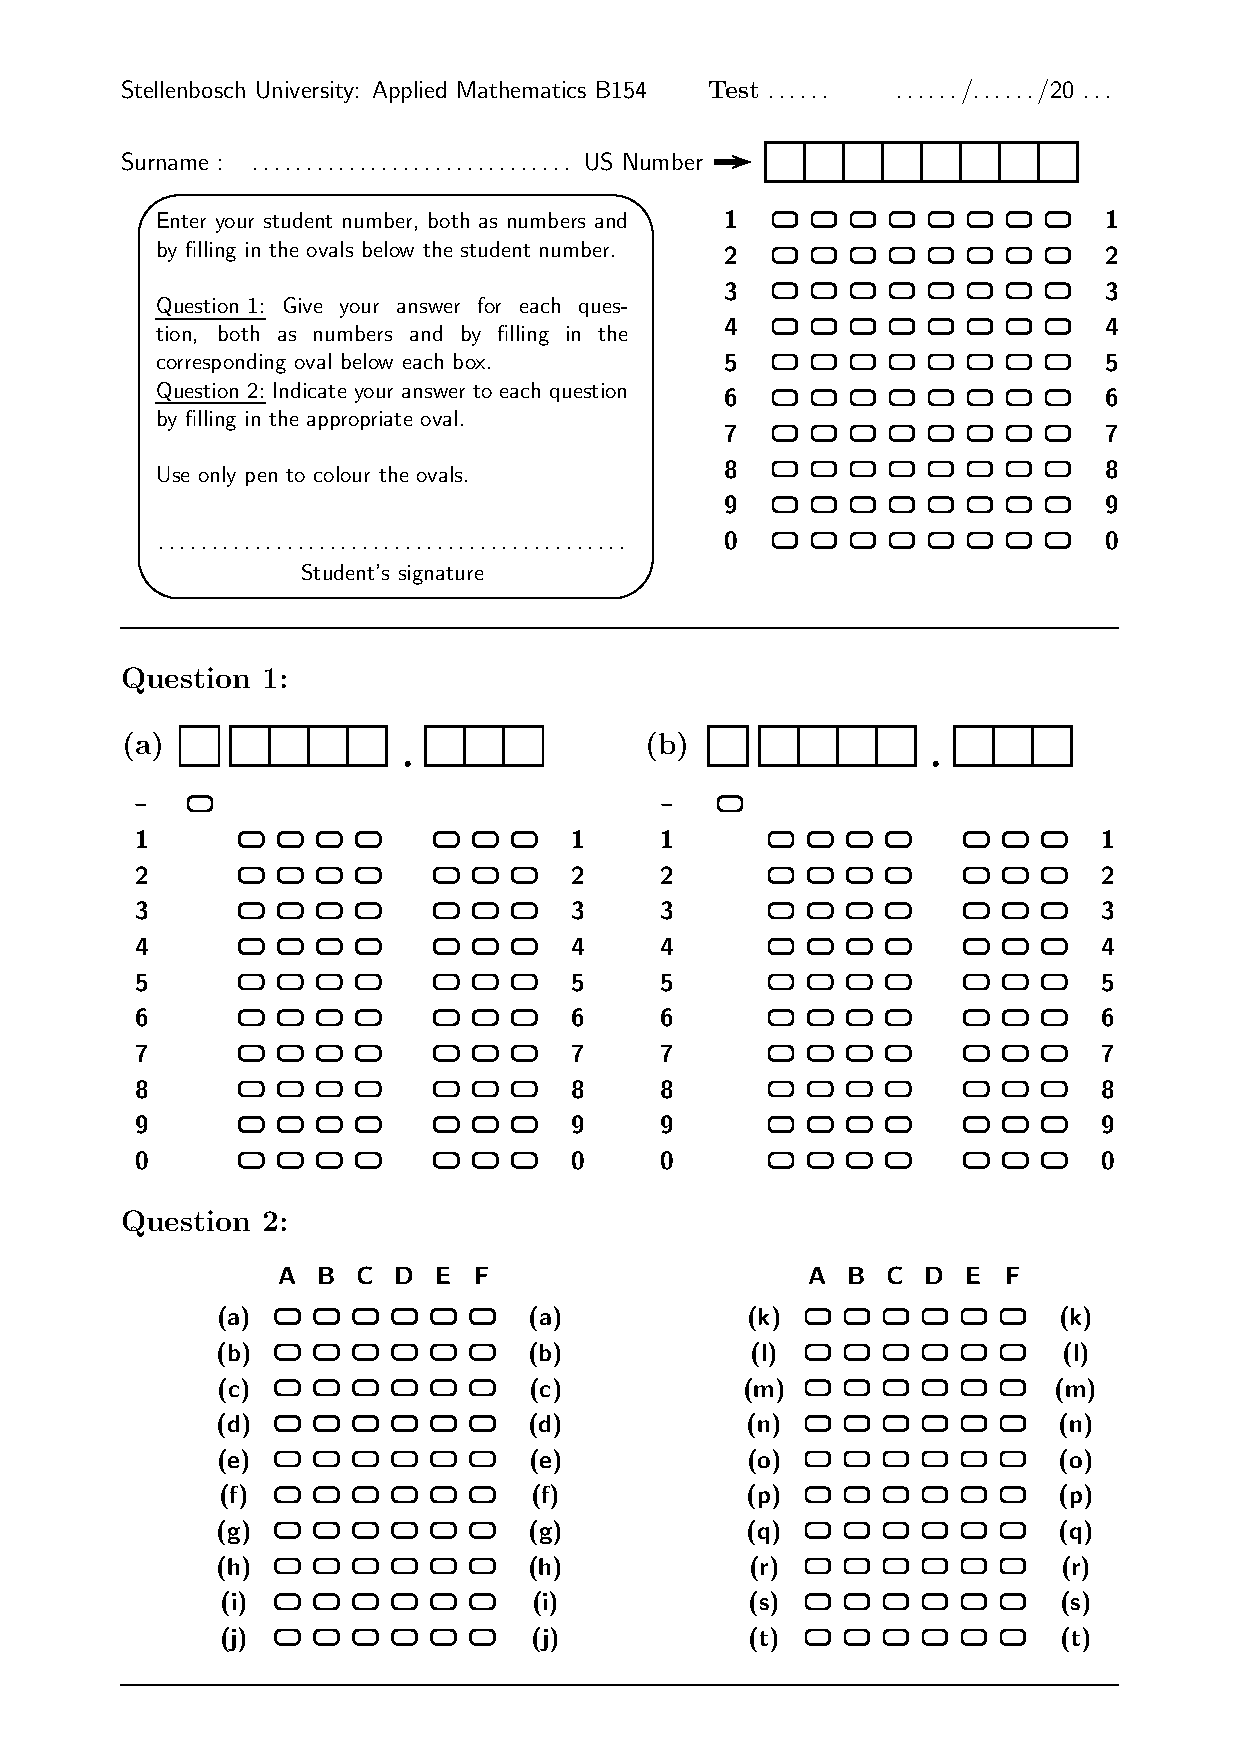
\includegraphics[width=8cm]{template2}\\
  \caption{Template allowing for numbered and multiple choice answers.}
  \label{fig:template2}
\end{figure}

\begin{figure}
  \centering
  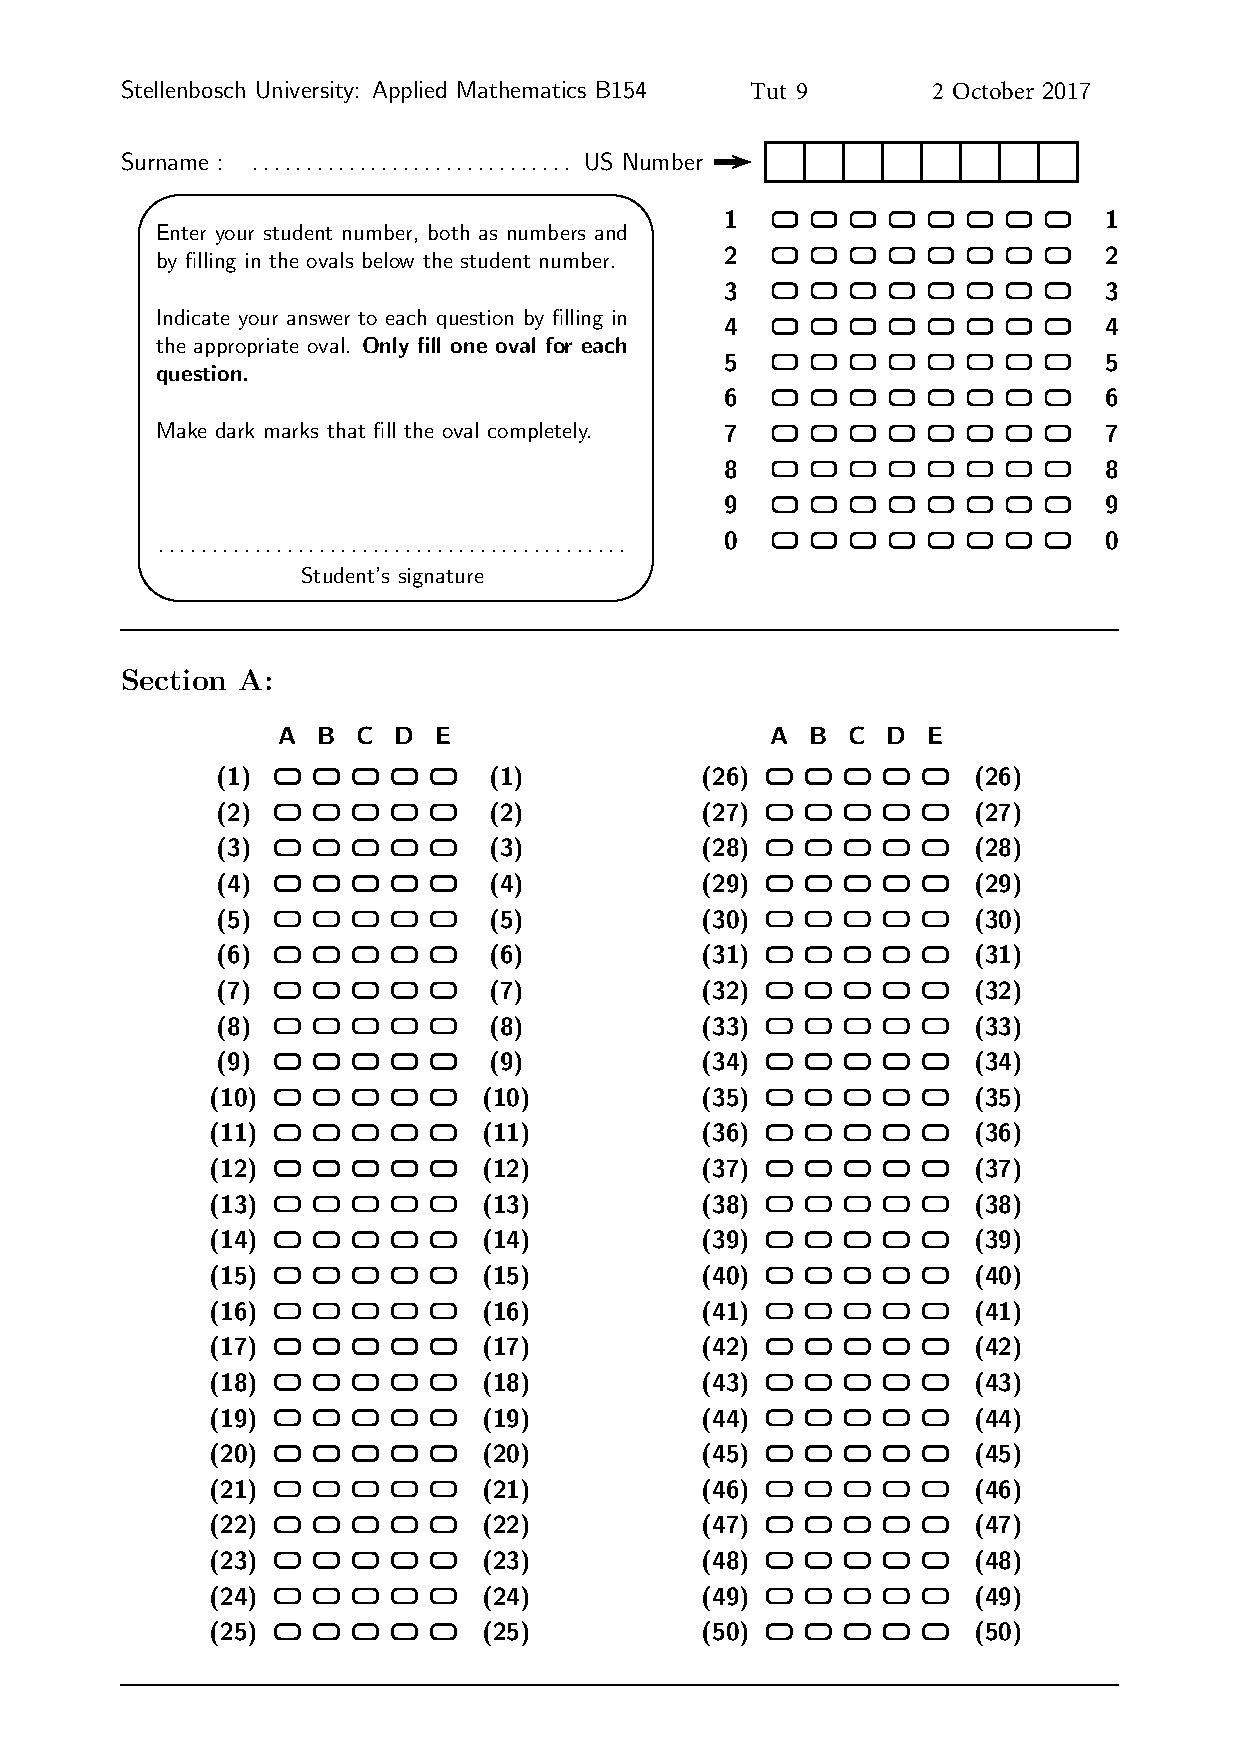
\includegraphics[width=8cm]{template3}\\
  \caption{Template focussed just on multiple choice type questions.}
  \label{fig:template3}
\end{figure}

\section{DCNN TensorFlow setup}
The DCNN structural setup diagram can be seen in Figure \ref{fig:DCNN}. This structure was directly used as constructed was constructed by the TensorFlow team.

\begin{figure}
  \centering
  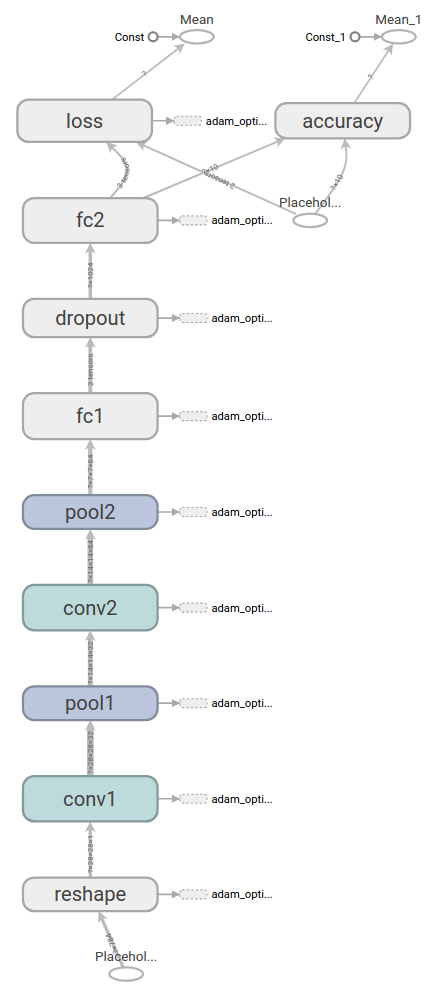
\includegraphics[width=8cm]{DCNN}\\
  \caption{DCNN structural setup diagram, from \citet{Tensor}}
  \label{fig:DCNN}
\end{figure}